% =====================================================================
%  core.tex  --  full core loaded geometry: the 8x9 lattice of cells, coloured
%  as in the MCNP render.  red = graphite (control cells), yellow = water (empty
%  cells, holes, rod gaps), green = aluminium, blue = UO2 fuel.  Holed control
%  cells show the central aluminium-lined water channel; fuel cells show their
%  4x4 inner lattice grid + rods, with the corner-empty (B3), half-filled (D4)
%  and middle-empty (F3) variants.  Columns A-H (top) and rows 1-9 (left, italic)
%  give the core coordinate system.
%  NB: the cell size is a fixed length (1.81 cm => ~0.95 of the 16 cm text width)
%  rather than a \textwidth fraction.  This is NOT \resizebox -- it only sets the
%  pgf coordinate unit, so fonts and line weights keep their true size.  The rod
%  and grid drawing is inlined (helper macros taking the rod coordinate triggered
%  a spurious "Dimension too large").  \input from chapters/2-geometry.tex.
% =====================================================================
\newcommand{\redcell}[2]{%
  \fill[yellow] (#1-1,9-#2) rectangle (#1,10-#2);
  \fill[red] (#1-0.951,9.049-#2) rectangle (#1-0.049,9.951-#2);
  \draw[thin] (#1-0.951,9.049-#2) rectangle (#1-0.049,9.951-#2);
  \draw (#1-1,9-#2) rectangle (#1,10-#2);}
\newcommand{\yellowcell}[2]{%
  \fill[yellow] (#1-1,9-#2) rectangle (#1,10-#2);
  \draw (#1-1,9-#2) rectangle (#1,10-#2);}
\newcommand{\holedcell}[2]{%
  \fill[yellow] (#1-1,9-#2) rectangle (#1,10-#2);
  \fill[red] (#1-0.951,9.049-#2) rectangle (#1-0.049,9.951-#2);
  \draw[thin] (#1-0.951,9.049-#2) rectangle (#1-0.049,9.951-#2);
  \fill[green!75!black] (#1-0.5,9.5-#2) circle (0.225);
  \draw[thin] (#1-0.5,9.5-#2) circle (0.225);
  \fill[yellow] (#1-0.5,9.5-#2) circle (0.20);
  \draw[thin] (#1-0.5,9.5-#2) circle (0.20);
  \draw (#1-1,9-#2) rectangle (#1,10-#2);}
\newcommand{\fuelbg}[2]{%
  \fill[yellow] (#1-1,9-#2) rectangle (#1,10-#2);
  \draw (#1-1,9-#2) rectangle (#1,10-#2);}
\newcommand{\rodgrid}[2]{%
  \begin{scope}[shift={(#1-0.5,9.5-#2)}]
    \draw[thin] (-0.451,-0.451) rectangle (0.451,0.451);
    \foreach \g in {-0.2257,0,0.2257}{
      \draw[thin] (\g,-0.451) -- (\g,0.451);
      \draw[thin] (-0.451,\g) -- (0.451,\g);}
    \foreach \dx in {-0.3385,-0.1128,0.1128,0.3385}
      \foreach \dy in {-0.3385,-0.1128,0.1128,0.3385}{
        \fill[green!75!black] (\dx,\dy) circle (0.072);
        \draw[thin] (\dx,\dy) circle (0.072);
        \fill[blue] (\dx,\dy) circle (0.046);
        \draw[thin] (\dx,\dy) circle (0.046);}
  \end{scope}}
\begin{figure}[H]
  \centering
  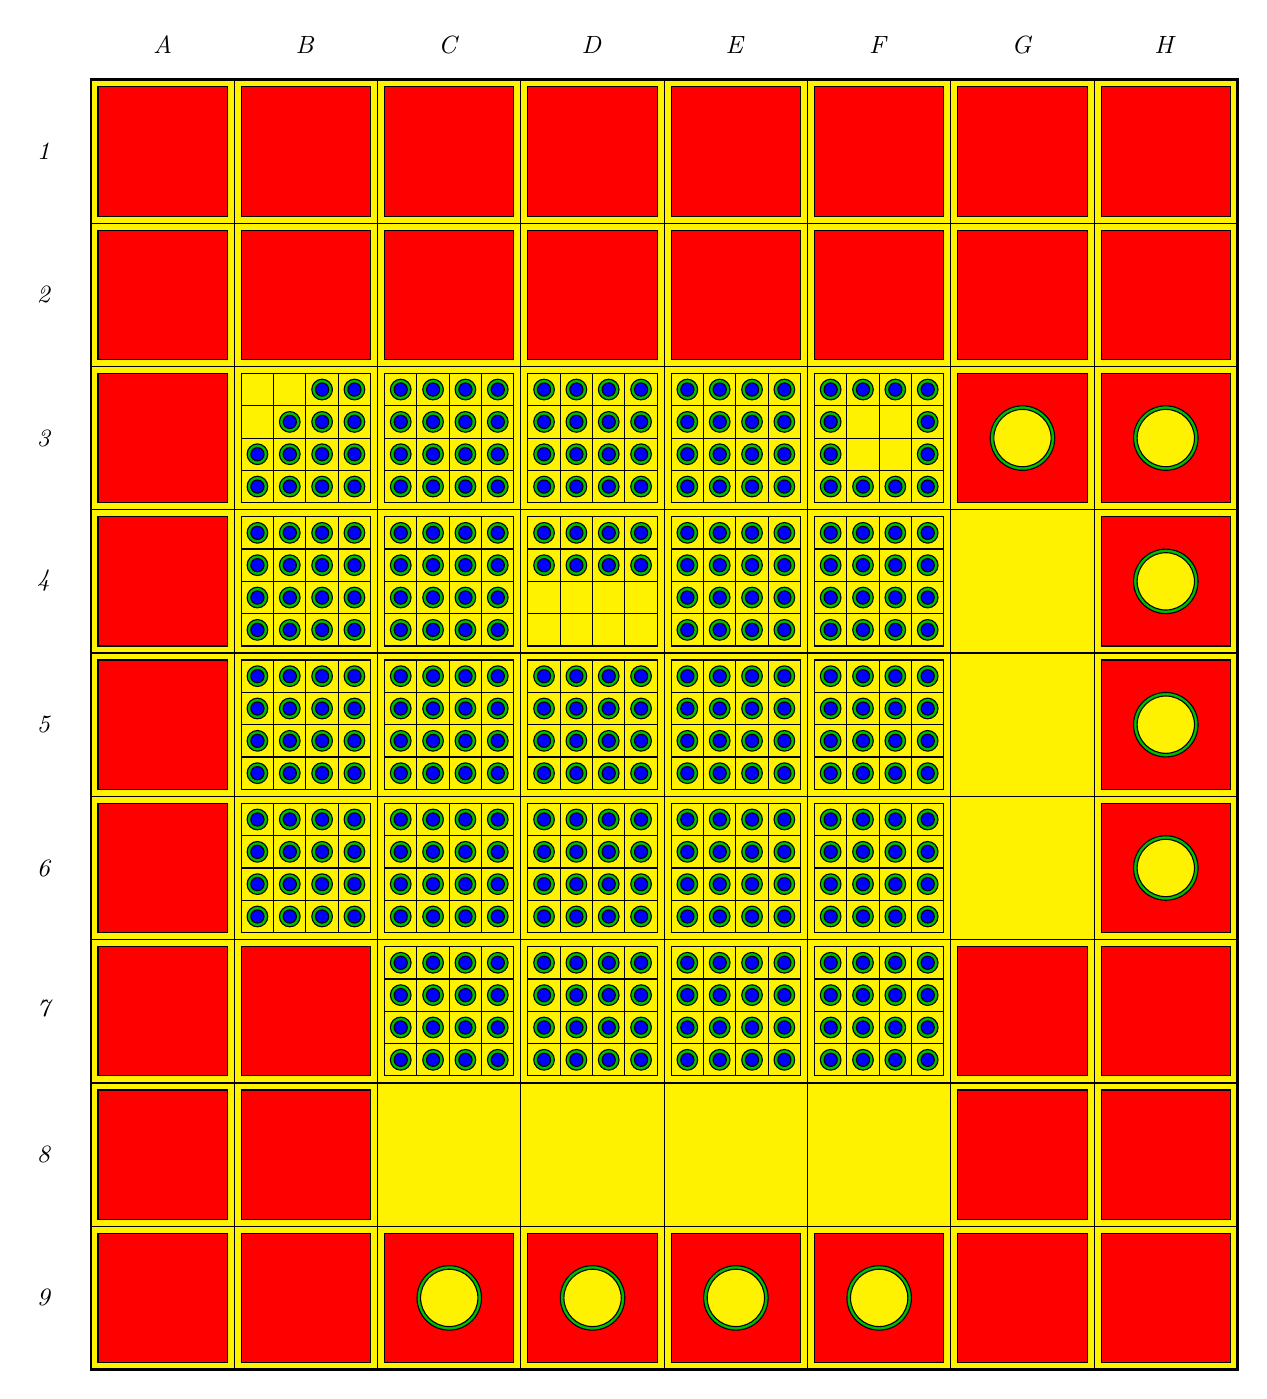
\begin{tikzpicture}[x=1.82cm,y=1.82cm,font=\small]
    \foreach \c/\r in {%
      1/1,2/1,3/1,4/1,5/1,6/1,7/1,8/1,%
      1/2,2/2,3/2,4/2,5/2,6/2,7/2,8/2,%
      1/3,1/4,1/5,1/6,%
      1/7,2/7,7/7,8/7,%
      1/8,2/8,7/8,8/8,%
      1/9,2/9,7/9,8/9}{\redcell{\c}{\r}}
    \foreach \c/\r in {7/4,7/5,7/6,3/8,4/8,5/8,6/8}{\yellowcell{\c}{\r}}
    \foreach \c/\r in {7/3,8/3,8/4,8/5,8/6,3/9,4/9,5/9,6/9}{\holedcell{\c}{\r}}
    \foreach \c/\r in {%
      3/3,4/3,5/3,%
      2/4,3/4,5/4,6/4,%
      2/5,3/5,4/5,5/5,6/5,%
      2/6,3/6,4/6,5/6,6/6,%
      3/7,4/7,5/7,6/7}{\fuelbg{\c}{\r}\rodgrid{\c}{\r}}
    % B3 corner-empty (col 2, row 3): top-left triangle has no rods
    \fuelbg{2}{3}
    \begin{scope}[shift={(1.5,6.5)}]
      \draw[thin] (-0.451,-0.451) rectangle (0.451,0.451);
      \foreach \g in {-0.2257,0,0.2257}{
        \draw[thin] (\g,-0.451) -- (\g,0.451);
        \draw[thin] (-0.451,\g) -- (0.451,\g);}
      \foreach \dx/\dy in {0.1128/0.3385,0.3385/0.3385,%
        -0.1128/0.1128,0.1128/0.1128,0.3385/0.1128,%
        -0.3385/-0.1128,-0.1128/-0.1128,0.1128/-0.1128,0.3385/-0.1128,%
        -0.3385/-0.3385,-0.1128/-0.3385,0.1128/-0.3385,0.3385/-0.3385}{
          \fill[green!75!black] (\dx,\dy) circle (0.072);
          \draw[thin] (\dx,\dy) circle (0.072);
          \fill[blue] (\dx,\dy) circle (0.046);
          \draw[thin] (\dx,\dy) circle (0.046);}
    \end{scope}
    % F3 middle-empty (col 6, row 3): inner 2x2 has no rods
    \fuelbg{6}{3}
    \begin{scope}[shift={(5.5,6.5)}]
      \draw[thin] (-0.451,-0.451) rectangle (0.451,0.451);
      \foreach \g in {-0.2257,0,0.2257}{
        \draw[thin] (\g,-0.451) -- (\g,0.451);
        \draw[thin] (-0.451,\g) -- (0.451,\g);}
      \foreach \dx/\dy in {-0.3385/0.3385,-0.1128/0.3385,0.1128/0.3385,0.3385/0.3385,%
        -0.3385/0.1128,0.3385/0.1128,%
        -0.3385/-0.1128,0.3385/-0.1128,%
        -0.3385/-0.3385,-0.1128/-0.3385,0.1128/-0.3385,0.3385/-0.3385}{
          \fill[green!75!black] (\dx,\dy) circle (0.072);
          \draw[thin] (\dx,\dy) circle (0.072);
          \fill[blue] (\dx,\dy) circle (0.046);
          \draw[thin] (\dx,\dy) circle (0.046);}
    \end{scope}
    % D4 half-filled (col 4, row 4): only the top two rows have rods
    \fuelbg{4}{4}
    \begin{scope}[shift={(3.5,5.5)}]
      \draw[thin] (-0.451,-0.451) rectangle (0.451,0.451);
      \foreach \g in {-0.2257,0,0.2257}{
        \draw[thin] (\g,-0.451) -- (\g,0.451);
        \draw[thin] (-0.451,\g) -- (0.451,\g);}
      \foreach \dx/\dy in {-0.3385/0.3385,-0.1128/0.3385,0.1128/0.3385,0.3385/0.3385,%
        -0.3385/0.1128,-0.1128/0.1128,0.1128/0.1128,0.3385/0.1128}{
          \fill[green!75!black] (\dx,\dy) circle (0.072);
          \draw[thin] (\dx,\dy) circle (0.072);
          \fill[blue] (\dx,\dy) circle (0.046);
          \draw[thin] (\dx,\dy) circle (0.046);}
    \end{scope}
    \draw[line width=1pt] (0,0) rectangle (8,9);
    \foreach \c/\L in {1/A,2/B,3/C,4/D,5/E,6/F,7/G,8/H}
      \node at (\c-0.5,9.24) {\textit{\L}};
    \foreach \r/\L in {1/1,2/2,3/3,4/4,5/5,6/6,7/7,8/8,9/9}
      \node at (-0.32,9.5-\r) {\textit{\L}};
  \end{tikzpicture}
  \caption{Reactor core geometry showing the lattice of cells. The colours represent materials, blue is UO$_2$ fuel, green is aluminum, yellow is water and red is graphite.}
  \label{fig:vised}
\end{figure}
